\section{Sets and Functions}

\subsection{Basic Set Theory}

%%%%%%%%%%%%%%%%%%%%%%%%%%%%%%%%% StartQuestion %%%%%%%%%%%%%%%%%%%%%%%%%%%%%%%%%%%%%%%%%%%%%%%5
\begin{question} 
	If $A, B$ and $C$ are sets. prove the followings:
	\begin{enumerate}[(a)]
		\item $A \cap (B \cup C) = (A \cap B) \cup (A \cap C)$. \label{section-a}
		\item $C \textbackslash (A \cup B) = (C \textbackslash A) \cap (C \backslash B)$.
		\item $C \backslash (A \cap B) = (C \backslash A) \cup (C \backslash B) $.
	\end{enumerate}
\end{question}
\begin{ans}
	\begin{enumerate}[(a)]
		\item 
		\begin{proof}
			Let $P, Q$, and $R$ be logical statements. We can show (using the truth table) that the following biconditional implication is a tautology. \[ P \wedge (Q \vee R) \Leftrightarrow (P \wedge Q) \vee (P \wedge R). \]
			Now let $x \in A \cap (B \cup C)$. Then $x \in A \wedge (x \in B \vee x \in C)$. Using the tautology above we can write $(x \in A \wedge x \in B) \vee (x \in A \wedge x \in C)$, thus $x \in (A \cap B) \cup (A \cap C) $, which means $A \cap (B \cap C) \subset (A \cap B) \cup (A \cap C)$. Conversely, let $x \in (A \cap B) \cup (A \cap C)$. By definition $(x \in A \wedge x \in B) \vee (x \in A \wedge x \in C)$. With the similar logic as above we can infer $(A \cap B) \cup (A \cap C) \subset A \cap (B \cup C)$. Thus $A \cap (B \cup C) = (A \cap B) \cup (A \cap C)$.
		\end{proof}
		
		\item 
		\begin{proof}
			Let $x \in C \backslash (A \cup B)$. By definition $x \in C \wedge x \notin (A \cup B) \biImp x \in C \wedge x \in \overline{A \cup B} \biImp x \in C \wedge x \in \bar{A} \cap \bar{B} \biImp x \in C \wedge (x \notin A \wedge x \notin B)$. Finally, using the following tautology 
			\[ P \wedge (Q \wedge R) \Leftrightarrow (P \wedge Q) \wedge (P \wedge R), \]
			we can write $(x \in C \wedge x \notin A) \wedge (x \in C \wedge x \notin B) \biImp x \in (C \backslash A) \cap (C \backslash B) $, thus $C \textbackslash (A \cup B) subset (C \textbackslash A) \cap (C \backslash B)$. The converse can be shown is true following the similar logic as below, thus inferring $C \textbackslash (A \cup B) = (C \textbackslash A) \cap (C \backslash B)$.
		\end{proof}
		
		\item \begin{proof}
			Let $x \in C \backslash (A \cap B)$. By definition $x \in C \wedge x \notin (A \cap B) \biImp x \in C \wedge x \in \overline{A \cap B} \biImp x \in C \wedge x \in \bar{A} \cup \bar{B} \biImp x \in C \wedge (x \notin A \vee x \notin B)$. Using the tautology in section (a),
			we can write $(x \in C \wedge x \notin A) \vee (x \in C \wedge x \notin B) \biImp x \in (C \backslash A) \cup (C \backslash B) $, thus $C \textbackslash (A \cap B) \subset (C \textbackslash A) \cup (C \backslash B)$. The converse can be shown is true following the similar logic as below, thus inferring $C \textbackslash (A \cap B) = (C \textbackslash A) \cup (C \backslash B)$.
		\end{proof}
	\end{enumerate}
\end{ans}
\newpage
%%%%%%%%%%%%%%%%%%%%%%%%%%%%%%%%% EndQuestion %%%%%%%%%%%%%%%%%%%%%%%%%%%%%%%%%%%%%%%%%%%%%%%5

\subsection{Functions}
%%%%%%%%%%%%%%%%%%%%%%%%%%%%%%%%% StartQuestion %%%%%%%%%%%%%%%%%%%%%%%%%%%%%%%%%%%%%%%%%%%%%%%5
\begin{question}
	\label{question:FunctionSetManipulation}
	Let $f: A \rightarrow B$. Let $C, C_1$, and $C_2$ be subsets of $A$, and let $D$ be a subset of $B$. Prove the followings. 
	\begin{enumerate}[(a)]
		\item If $f$ is one-to-one, then $f(C_1 \cap C_2) = f(C_1) \cap f(C_2)$.
		\item If $f$ is one-to-one, then $f^{-1}(f(C))=C$.
		\item If $f$ is onto, then $f(\preIm{f}(D)) = D$. 
	\end{enumerate}
\end{question}
\begin{ans}
	\begin{enumerate}[(a)]
		\item 
		\begin{proof}
			Let $C_1, C_2 \in A$. Then $f(C_1 \cap C_2) = \{ y \in B : y = f(x), x \in C_1 \cap C_2 \} = \{  y \in B : y = f(x), x \in C_1 \wedge x \in C_2 \}$. Let $\tilde{y} \in f(C_1 \cap C_2)$. Then from the definition above, $\tilde{y} = f(\tilde{x}) \quad \text{s.t.} \quad \tilde{x} \in C_1 \wedge \tilde{x} \in C_2 $. Using the definition of function, we can write $\tilde{y} \in f(C_1) \wedge \tilde{y} \in f(C_2) \biImp \tilde{y} \in f(C_1) \cap f(C_2)$. Thus $f(C_1 \cap C_2) \subset f(C_1) \cap f(C_2)$. Conversely, let $y \in (f(C_1) \cap f(C_2))$. Then by definition
			\begin{align*}
				y \in f(C_1) \Rightarrow \exists x_1 \in C_1 \st y = f(x_1), \\
				y \in f(C_2) \Rightarrow \exists x_2 \in C_2 \st y = f(x_2). 
			\end{align*}
			Since $f$ is one-to-one, then $f(x_1) = f(x_2) \Rightarrow x = x_1 = x_2$. Thus $x \in C_1 \cap C_2, y = f(x) \in f(C_1 \cap C_2)$. So $f(C_1) \cap f(C_2) \subset f(C_1) \cap f(C_2)$. Finally we can conclude $f(C_1 \cap C_2) = f(C_1) \cap f(C_2)$.
		\end{proof}
		\item 
		\begin{proof}
			Let $C \in A$, and $a \in f^{-1}(f(C))$. Since $f^{-1}(f(C)) = \{ x \in A: f(x) \in f(C) \}$, then $f(a) \in f(C)$. Thus $\exists x_c \in C \st f(a) = f(x_c)$. Since $f$ is one-to-one, then $a = x_c \biImp a \in C$. So we will have $f^{-1}(f(C)) \subset C$ .Conversely, let $a \in C$. Then by definition $f(a) \in f(C) \biImp f(a) \in f^{-1}(f(C))$. So $C \subset f^{-1}(f(C)) $. So we can conclude $f^{-1}(f(C))=C$.
		\end{proof}
		\item 
		\begin{proof}
			Let $D \subset B$, $b \in D$. Since $f$ is onto, then $\exists a \in A \st b = f(a)$, thus $a \in \preIm{f}(D)$. And by definition $b \in f(\preIm{f}(D))$, thus $D \subset f(\preIm{f}(D))$. Conversely, Let $b \in f(\preIm{f}(D))$. Then $\exists a \in \preIm{f}(D) \st f(a)=b $, hence from definition it follows that $b \in D$, implying $f(\preIm{f}(D)) \subset D$. So we conclude that $f(\preIm{f}(D)) = D$.
		\end{proof}
	\end{enumerate}
\end{ans}
\newpage
%%%%%%%%%%%%%%%%%%%%%%%%%%%%%%%%% EndQuestion %%%%%%%%%%%%%%%%%%%%%%%%%%%%%%%%%%%%%%%%%%%%%%%

%%%%%%%%%%%%%%%%%%%%%%%%%%%%%%%%% StartQuestion %%%%%%%%%%%%%%%%%%%%%%%%%%%%%%%%%%%%%%%%%%%%%%%5
\begin{question}
	For all sub-sections of Question \autoref{question:FunctionSetManipulation} construct a specific example in which the indicated equation fails. (Of course the given hypothesis will have to be false too.)
\end{question}
\begin{ans}
	\begin{enumerate}[(a)]
		\item \text{\\include{Q4a.tex}}
		\item From the figure below, it is clear that $\tilde{x} \in \preIm{f}(f(C))$ but $\tilde{x} \notin C$, thus $\preIm{f}(f(C)) \nsubset C$.
		\begin{figure}[h!]
	\centering
	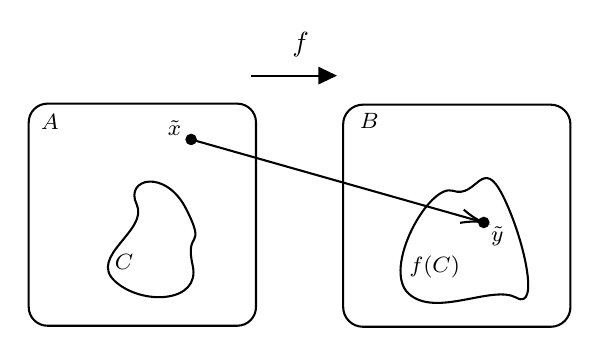
\begin{tikzpicture}[x=0.75pt,y=0.75pt,yscale=-1,xscale=1]
		%uncomment if require: \path (0,300); %set diagram left start at 0, and has height of 300
		
		%Rounded Rect [id:dp0586838643025005] 
		\draw   (50,73) .. controls (50,68.03) and (54.03,64) .. (59,64) -- (150.5,64) .. controls (155.47,64) and (159.5,68.03) .. (159.5,73) -- (159.5,162) .. controls (159.5,166.97) and (155.47,171) .. (150.5,171) -- (59,171) .. controls (54.03,171) and (50,166.97) .. (50,162) -- cycle ;
		%Rounded Rect [id:dp40936794872995397] 
		\draw   (201.5,74) .. controls (201.5,68.75) and (205.75,64.5) .. (211,64.5) -- (301.5,64.5) .. controls (306.75,64.5) and (311,68.75) .. (311,74) -- (311,162) .. controls (311,167.25) and (306.75,171.5) .. (301.5,171.5) -- (211,171.5) .. controls (205.75,171.5) and (201.5,167.25) .. (201.5,162) -- cycle ;
		%Shape: Polygon Curved [id:ds8529440642936859] 
		\draw   (102,112.5) .. controls (96,100) and (116,95) .. (126,115) .. controls (136,135) and (125,124) .. (129,142) .. controls (133,160) and (104.5,161.5) .. (91.5,149.5) .. controls (78.5,137.5) and (108,125) .. (102,112.5) -- cycle ;
		%Shape: Polygon Curved [id:ds16879268501997946] 
		\draw   (254.5,106) .. controls (266,110) and (268.5,88.5) .. (278.5,108.5) .. controls (288.5,128.5) and (296.5,164) .. (285,157.5) .. controls (273.5,151) and (246,167.5) .. (233,155.5) .. controls (220,143.5) and (243,102) .. (254.5,106) -- cycle ;
		%Shape: Circle [id:dp10126802720694927] 
		\draw  [color={rgb, 255:red, 0; green, 0; blue, 0 }  ,draw opacity=1 ][fill={rgb, 255:red, 0; green, 0; blue, 0 }  ,fill opacity=1 ] (126,81.25) .. controls (126,80.01) and (127.01,79) .. (128.25,79) .. controls (129.49,79) and (130.5,80.01) .. (130.5,81.25) .. controls (130.5,82.49) and (129.49,83.5) .. (128.25,83.5) .. controls (127.01,83.5) and (126,82.49) .. (126,81.25) -- cycle ;
		%Shape: Circle [id:dp5328965179835532] 
		\draw  [color={rgb, 255:red, 0; green, 0; blue, 0 }  ,draw opacity=1 ][fill={rgb, 255:red, 0; green, 0; blue, 0 }  ,fill opacity=1 ] (267,121.25) .. controls (267,120.01) and (268.01,119) .. (269.25,119) .. controls (270.49,119) and (271.5,120.01) .. (271.5,121.25) .. controls (271.5,122.49) and (270.49,123.5) .. (269.25,123.5) .. controls (268.01,123.5) and (267,122.49) .. (267,121.25) -- cycle ;
		%Straight Lines [id:da5038858731694382] 
		\draw    (157,50.5) -- (195.5,50.5) ;
		\draw [shift={(198.5,50.5)}, rotate = 180] [fill={rgb, 255:red, 0; green, 0; blue, 0 }  ][line width=0.08]  [draw opacity=0] (8.93,-4.29) -- (0,0) -- (8.93,4.29) -- cycle    ;
		%Straight Lines [id:da30392969256002633] 
		\draw    (128.25,81.25) -- (267.33,120.7) ;
		\draw [shift={(269.25,121.25)}, rotate = 195.84] [color={rgb, 255:red, 0; green, 0; blue, 0 }  ][line width=0.75]    (10.93,-3.29) .. controls (6.95,-1.4) and (3.31,-0.3) .. (0,0) .. controls (3.31,0.3) and (6.95,1.4) .. (10.93,3.29)   ;
		
		% Text Node
		\draw (90,135) node [anchor=north west][inner sep=0.75pt]  [font=\footnotesize] [align=left] {$\displaystyle C$};
		% Text Node
		\draw (54.5,67.5) node [anchor=north west][inner sep=0.75pt]  [font=\footnotesize] [align=left] {$\displaystyle A$};
		% Text Node
		\draw (208,67) node [anchor=north west][inner sep=0.75pt]  [font=\footnotesize] [align=left] {$\displaystyle B$};
		% Text Node
		\draw (232,136) node [anchor=north west][inner sep=0.75pt]  [font=\footnotesize] [align=left] {$\displaystyle f( C)$};
		% Text Node
		\draw (115.5,70.5) node [anchor=north west][inner sep=0.75pt]  [font=\footnotesize] [align=left] {$\displaystyle \tilde{x}$};
		% Text Node
		\draw (271.25,122) node [anchor=north west][inner sep=0.75pt]  [font=\footnotesize] [align=left] {$\displaystyle \tilde{y}$};
		% Text Node
		\draw (175.5,27.9) node [anchor=north west][inner sep=0.75pt]    {$f$};
		
		
	\end{tikzpicture}
	
	
	
\end{figure}
	
		\item In the figure below, the set $\tilde{D} \subset D$, shown as a shaded region, has not been mapped (since we assume that $f$ is not onto). Then for any $b \in \tilde{D}$ we have $b \notin f(\preIm{f}(D))$, thus $D \nsubset f(\preIm{f}(D))$.
		

\begin{figure}[h!]
	\centering
	\tikzset{
		pattern size/.store in=\mcSize, 
		pattern size = 5pt,
		pattern thickness/.store in=\mcThickness, 
		pattern thickness = 0.3pt,
		pattern radius/.store in=\mcRadius, 
		pattern radius = 1pt}
	\makeatletter
	\pgfutil@ifundefined{pgf@pattern@name@_ngjcsk6nk}{
		\pgfdeclarepatternformonly[\mcThickness,\mcSize]{_ngjcsk6nk}
		{\pgfqpoint{0pt}{0pt}}
		{\pgfpoint{\mcSize+\mcThickness}{\mcSize+\mcThickness}}
		{\pgfpoint{\mcSize}{\mcSize}}
		{
			\pgfsetcolor{\tikz@pattern@color}
			\pgfsetlinewidth{\mcThickness}
			\pgfpathmoveto{\pgfqpoint{0pt}{0pt}}
			\pgfpathlineto{\pgfpoint{\mcSize+\mcThickness}{\mcSize+\mcThickness}}
			\pgfusepath{stroke}
	}}
	\makeatother
	\tikzset{every picture/.style={line width=0.75pt}} %set default line width to 0.75pt        
	
	\begin{tikzpicture}[x=0.75pt,y=0.75pt,yscale=-1,xscale=1]
		%uncomment if require: \path (0,300); %set diagram left start at 0, and has height of 300
		
		%Rounded Rect [id:dp21367529792537088] 
		\draw   (70,93) .. controls (70,88.03) and (74.03,84) .. (79,84) -- (170.5,84) .. controls (175.47,84) and (179.5,88.03) .. (179.5,93) -- (179.5,182) .. controls (179.5,186.97) and (175.47,191) .. (170.5,191) -- (79,191) .. controls (74.03,191) and (70,186.97) .. (70,182) -- cycle ;
		%Rounded Rect [id:dp651427111410396] 
		\draw   (221.5,94) .. controls (221.5,88.75) and (225.75,84.5) .. (231,84.5) -- (321.5,84.5) .. controls (326.75,84.5) and (331,88.75) .. (331,94) -- (331,182) .. controls (331,187.25) and (326.75,191.5) .. (321.5,191.5) -- (231,191.5) .. controls (225.75,191.5) and (221.5,187.25) .. (221.5,182) -- cycle ;
		%Shape: Polygon Curved [id:ds6468442929460672] 
		\draw   (122,132.5) .. controls (137.5,142.5) and (136,115) .. (146,135) .. controls (156,155) and (170,165) .. (155.5,173) .. controls (141,181) and (103.5,187) .. (90.5,175) .. controls (77.5,163) and (106.5,122.5) .. (122,132.5) -- cycle ;
		%Shape: Polygon Curved [id:ds2558075497670429] 
		\draw   (251.5,122) .. controls (263,126) and (288.5,104) .. (298.5,124) .. controls (308.5,144) and (335,156.5) .. (309.5,168) .. controls (284,179.5) and (266,183) .. (253,171) .. controls (240,159) and (240,118) .. (251.5,122) -- cycle ;
		%Straight Lines [id:da7883937235787493] 
		\draw    (177,70.5) -- (215.5,70.5) ;
		\draw [shift={(218.5,70.5)}, rotate = 180] [fill={rgb, 255:red, 0; green, 0; blue, 0 }  ][line width=0.08]  [draw opacity=0] (8.93,-4.29) -- (0,0) -- (8.93,4.29) -- cycle    ;
		%Shape: Polygon Curved [id:ds7055583197786395] 
		\draw  [pattern=_ngjcsk6nk,pattern size=3.6750000000000003pt,pattern thickness=0.75pt,pattern radius=0pt, pattern color={rgb, 255:red, 0; green, 0; blue, 0}] (296.5,144.5) .. controls (301,145.5) and (304,146.5) .. (310.5,146.5) .. controls (317,146.5) and (322.5,155.5) .. (319.5,160.5) .. controls (316.5,165.5) and (296,160.5) .. (293.5,155.5) .. controls (291,150.5) and (292,143.5) .. (296.5,144.5) -- cycle ;
		
		% Text Node
		\draw (90.5,154.5) node [anchor=north west][inner sep=0.75pt]  [font=\scriptsize] [align=left] {$\displaystyle f^{1}( D)$};
		% Text Node
		\draw (74.5,87.5) node [anchor=north west][inner sep=0.75pt]  [font=\footnotesize] [align=left] {$\displaystyle A$};
		% Text Node
		\draw (228,87) node [anchor=north west][inner sep=0.75pt]  [font=\footnotesize] [align=left] {$\displaystyle B$};
		% Text Node
		\draw (195.5,47.9) node [anchor=north west][inner sep=0.75pt]    {$f$};
		% Text Node
		\draw (245.5,125) node [anchor=north west][inner sep=0.75pt]  [font=\footnotesize] [align=left] {$\displaystyle D$};
		% Text Node
		\draw (282,149.5) node [anchor=north west][inner sep=0.75pt]  [font=\tiny] [align=left] {$\displaystyle \tilde{D}$};
		
		
	\end{tikzpicture}
\end{figure}


	\end{enumerate}
\end{ans}
%%%%%%%%%%%%%%%%%%%%%%%%%%%%%%%%% EndQuestion %%%%%%%%%%%%%%%%%%%%%%%%%%%%%%%%%%%%%%%%%%%%%%%
\newpage
%%%%%%%%%%%%%%%%%%%%%%%%%%%%%%%%% StartQuestion %%%%%%%%%%%%%%%%%%%%%%%%%%%%%%%%%%%%%%%%%%%%%%%5
\begin{question}
	{Question 8}. Let $f: A \rightarrow B$ and let $C \subseteq A$. Answer the followings.
	\begin{enumerate}[(a)]
		\item Proof or counterexample: $f(A\backslash C) \subseteq f(A) \backslash f(C)$.
		\item Proof or counterexample: $f(A\backslash C) \supseteq f(A) \backslash f(C)$.	
		\item What condition on $f$ will guarantee $f(A\backslash C) = f(A) \backslash f(C)$. \\

	\end{enumerate}
	\begin{ans}
		\begin{enumerate}[(a)]
			\item \begin{proof}
				Let $y \in B \st y \in f(A \backslash C)$. From definition $y = f(\tilde{x})\ \text{for some}\ \tilde{x} \in A \backslash C \biImp \tilde{x} \in A \wedge \tilde{x} \notin C$. Now construct the function in a way that $\exists x_c \in C \st f(x_c) = f(\tilde{x})$. Thus $f$ is \textbf{not} \oo. So $y = f(\tilde{x}) = f(x_c) \in f(C)$. We can write:
				\begin{align*}
					y &\in f(C), \\
					y &\in f(C) \cup \overline{f(A)}, \\
					y &\in \overline{(\overline{f(C)} \cap f(A))}, \\
					y &\notin \overline{f(C)} \cap f(A),\\
					y &\notin f(A) \backslash f(C).
				\end{align*}
				Thus $f(A\backslash C) \nsubset f(A) \backslash f(C)$.
			\end{proof}
			
			\item \begin{proof}
				Let $y \in B \st y \in f(A) \backslash f(C)$. So $y \in f(A) \wedge y \notin f(C)$. From definition $y = f(x_1)$ for some $x_1 \in A$ and $y = f(x_2)$ for some $x_2 \notin C$. Then if $f$ is \oo, $y=f(x_1) = f(x_2) \Rightarrow x = x_1 = x_2$, in which $x \in A \wedge x \notin C$, hence $x \in A\backslash C$. So from definition $y \in f(A\backslash C)$ which implies $f(A\backslash C) \supseteq f(A) \backslash f(C)$.
			\end{proof}
			
			\item $f$ should be \oo to guarantee $f(A\backslash C) = f(A) \backslash f(C)$. Proof is provided in (a) and (b).
		\end{enumerate}
	\end{ans}
\end{question}
\newpage
%%%%%%%%%%%%%%%%%%%%%%%%%%%%%%%%% EndQuestion %%%%%%%%%%%%%%%%%%%%%%%%%%%%%%%%%%%%%%%%%%%%%%%

%%%%%%%%%%%%%%%%%%%%%%%%%%%%%%%%% StartQuestion %%%%%%%%%%%%%%%%%%%%%%%%%%%%%%%%%%%%%%%%%%%%%%%
\begin{question}
	\begin{enumerate}[(a)]
		\item Suppose $f: X \rightarrow X$ is a function, and define $g=f \o f$. Prove: if $g(x)=x$ for all $x \in X$, then $f$ is \oo and onto.
		\item Extend the results in (a) to the function $g = f \o f \o \hdots \o f$ defined by compositing $f$ by itself $n$ times. Show that the results is valid for each $n \in \N$.
	\end{enumerate}
\end{question}

\begin{ans}
	\begin{enumerate}[(a)]
		\item 
		\begin{proof}
			Lets first prove that $f$ is \oo. Let $x_1 \neq x_2 \in X \st f(x_1) = f(x_2)$. By definition $f(f(x_1)) = f(f(x_2)) \biImp g(x_1) = g(x_2) \biImp x_1 = x_2$, thus $f$ is \oo.
			
			Now we prove that $f$ is onto. $\forall y \in X$, setting $x=f(y)\in X$ will yield $y = f(x) = f(f(y)) = g(y) = y$. Thus $f$ is onto.
		\end{proof}
		\item 
		\begin{proof}
			First we prove that $f$ is \oo.  Let $x_1 \neq x_2 \in X \st f(x_1) = f(x_2)$. By definition $f(f(x_1)) = f(f(x_2)) \biImp f(f(f(x_1))) = f(f(f(x_2))) \biImp  f(f(\hdots f(x_2) \hdots)) = f(f(\hdots f(x_1) \hdots)) \biImp g(x_1) = g(x_2) \biImp x_1 = x_2$, thus $f$ is \oo.
			
			Now we prove that $f$ is onto. $\forall y \in X$, setting $x=(\overbrace{f \o f \o \hdots \o f}^{n-1})(y)\in X$ will yield $y = f(x) = (\overbrace{f \o f \o \hdots \o f}^{n})(y) = g(y) = y$. Thus $f$ is onto.
			
			Now by induction we can infer that this is true $\forall n \in \N$.
		\end{proof}
	\end{enumerate}
\end{ans}
\newpage
%%%%%%%%%%%%%%%%%%%%%%%%%%%%%%%%% EndQuestion %%%%%%%%%%%%%%%%%%%%%%%%%%%%%%%%%%%%%%%%%%%%%%%


%%%%%%%%%%%%%%%%%%%%%%%%%%%%%%%%% StartQuestion %%%%%%%%%%%%%%%%%%%%%%%%%%%%%%%%%%%%%%%%%%%%%%%
\begin{question}
	Let $f: A \rightarrow B$ and $g: B \rightarrow C$ be given functions. Use the symbol $g \circ f$ to denote the function from $A$ to $C$ defined by $(g \circ f)(x) = g(f(x))$ for all $x \in A$. Prove the followings. 
	
	\begin{enumerate}[(a)]
		\item If $f$ and $g$ are one-to-one, then $g \circ f$ is one-to-one.
		\item If $g \o f$ is \oo, then $f$ is \oo.
		\item If $f$ is onto and $g \o f$ is \oo, then $g$ is \oo.
		\item It can happen that $g \o f$ is \oo, but $g$ is not. 
	\end{enumerate}
\end{question}
\begin{ans}
	\begin{enumerate}[(a)]
		\item \begin{proof}
			Let $x_1 \neq x_2 \in A \st (g \o f)(x_1)  = (g \o f)(x_2)$. Since $g$ is \oo then $f(x_2) = f(x_1)$. Similarly, since $f$ is \oo, then $x_1 = x_2$, hence $g \o f$ is \oo.
		\end{proof}
		\item \begin{proof}
			Let $x_1 \neq x_2 \in A \st f(x_1) = f(x_2)$. By definition of a function we can write $g(f(x_1)) = g(f(x_2)) \biImp (g \o f)(x_1) = (g \o f)(x_2)$. Since $g \o f$ is \oo, then $x_1 = x_2$. This then implies that  $f$ is \oo. 
		\end{proof}
		\item \begin{proof}
			Let $b_1 \neq b_2 \in B \st g(b_1) = g(b_2)$. Since $f$ is onto, then for $b_1, b_2 \in B, \exists a_1, a_2 \in A, \st b_1 = f(a_1), b_2 = f(a_2)$. So we can write $g(f(a_1)) = g(f(a_2))$. Since $g \o f$ is \oo, $a_1 = a_2$. From definition of a function it follows $b_1 = f(a_1) = f(a_2) = b_2$, hence implies $g$ is \oo.
		\end{proof}
		\item \begin{proof}
			The following figure shows a specific example in which $g \o f$ is \oo, however $g$ is not. 
			\begin{figure}[h!]
	\centering
	\tikzset{every picture/.style={line width=0.75pt}} %set default line width to 0.75pt        
	
	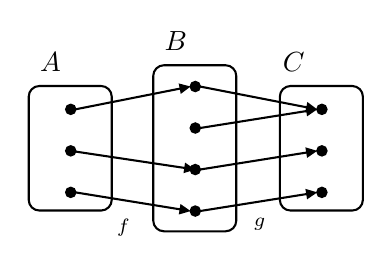
\begin{tikzpicture}[x=0.75pt,y=0.75pt,yscale=-1,xscale=1]
		%uncomment if require: \path (0,300); %set diagram left start at 0, and has height of 300
		
		%Rounded Rect [id:dp17761622576856428] 
		\draw   (90,45.14) .. controls (90,42.3) and (92.3,40) .. (95.14,40) -- (124.86,40) .. controls (127.7,40) and (130,42.3) .. (130,45.14) -- (130,94.86) .. controls (130,97.7) and (127.7,100) .. (124.86,100) -- (95.14,100) .. controls (92.3,100) and (90,97.7) .. (90,94.86) -- cycle ;
		%Rounded Rect [id:dp46557282862056737] 
		\draw   (150,35.14) .. controls (150,32.3) and (152.3,30) .. (155.14,30) -- (184.86,30) .. controls (187.7,30) and (190,32.3) .. (190,35.14) -- (190,104.86) .. controls (190,107.7) and (187.7,110) .. (184.86,110) -- (155.14,110) .. controls (152.3,110) and (150,107.7) .. (150,104.86) -- cycle ;
		%Shape: Circle [id:dp19422500705460033] 
		\draw  [fill={rgb, 255:red, 0; green, 0; blue, 0 }  ,fill opacity=1 ] (108,51.25) .. controls (108,50.01) and (109.01,49) .. (110.25,49) .. controls (111.49,49) and (112.5,50.01) .. (112.5,51.25) .. controls (112.5,52.49) and (111.49,53.5) .. (110.25,53.5) .. controls (109.01,53.5) and (108,52.49) .. (108,51.25) -- cycle ;
		%Shape: Circle [id:dp4181725904000142] 
		\draw  [fill={rgb, 255:red, 0; green, 0; blue, 0 }  ,fill opacity=1 ] (108,71.25) .. controls (108,70.01) and (109.01,69) .. (110.25,69) .. controls (111.49,69) and (112.5,70.01) .. (112.5,71.25) .. controls (112.5,72.49) and (111.49,73.5) .. (110.25,73.5) .. controls (109.01,73.5) and (108,72.49) .. (108,71.25) -- cycle ;
		%Shape: Circle [id:dp14173404339102347] 
		\draw  [fill={rgb, 255:red, 0; green, 0; blue, 0 }  ,fill opacity=1 ] (108,91.25) .. controls (108,90.01) and (109.01,89) .. (110.25,89) .. controls (111.49,89) and (112.5,90.01) .. (112.5,91.25) .. controls (112.5,92.49) and (111.49,93.5) .. (110.25,93.5) .. controls (109.01,93.5) and (108,92.49) .. (108,91.25) -- cycle ;
		%Shape: Circle [id:dp5562995636986945] 
		\draw  [fill={rgb, 255:red, 0; green, 0; blue, 0 }  ,fill opacity=1 ] (168,40.25) .. controls (168,39.01) and (169.01,38) .. (170.25,38) .. controls (171.49,38) and (172.5,39.01) .. (172.5,40.25) .. controls (172.5,41.49) and (171.49,42.5) .. (170.25,42.5) .. controls (169.01,42.5) and (168,41.49) .. (168,40.25) -- cycle ;
		%Shape: Circle [id:dp5009502155253602] 
		\draw  [fill={rgb, 255:red, 0; green, 0; blue, 0 }  ,fill opacity=1 ] (168,60.25) .. controls (168,59.01) and (169.01,58) .. (170.25,58) .. controls (171.49,58) and (172.5,59.01) .. (172.5,60.25) .. controls (172.5,61.49) and (171.49,62.5) .. (170.25,62.5) .. controls (169.01,62.5) and (168,61.49) .. (168,60.25) -- cycle ;
		%Shape: Circle [id:dp5804192548416451] 
		\draw  [fill={rgb, 255:red, 0; green, 0; blue, 0 }  ,fill opacity=1 ] (168,80.25) .. controls (168,79.01) and (169.01,78) .. (170.25,78) .. controls (171.49,78) and (172.5,79.01) .. (172.5,80.25) .. controls (172.5,81.49) and (171.49,82.5) .. (170.25,82.5) .. controls (169.01,82.5) and (168,81.49) .. (168,80.25) -- cycle ;
		%Shape: Circle [id:dp09763005580799611] 
		\draw  [fill={rgb, 255:red, 0; green, 0; blue, 0 }  ,fill opacity=1 ] (168,100.25) .. controls (168,99.01) and (169.01,98) .. (170.25,98) .. controls (171.49,98) and (172.5,99.01) .. (172.5,100.25) .. controls (172.5,101.49) and (171.49,102.5) .. (170.25,102.5) .. controls (169.01,102.5) and (168,101.49) .. (168,100.25) -- cycle ;
		%Rounded Rect [id:dp7702902675019128] 
		\draw   (211,45.14) .. controls (211,42.3) and (213.3,40) .. (216.14,40) -- (245.86,40) .. controls (248.7,40) and (251,42.3) .. (251,45.14) -- (251,94.86) .. controls (251,97.7) and (248.7,100) .. (245.86,100) -- (216.14,100) .. controls (213.3,100) and (211,97.7) .. (211,94.86) -- cycle ;
		%Shape: Circle [id:dp7132439025228492] 
		\draw  [fill={rgb, 255:red, 0; green, 0; blue, 0 }  ,fill opacity=1 ] (229,51.25) .. controls (229,50.01) and (230.01,49) .. (231.25,49) .. controls (232.49,49) and (233.5,50.01) .. (233.5,51.25) .. controls (233.5,52.49) and (232.49,53.5) .. (231.25,53.5) .. controls (230.01,53.5) and (229,52.49) .. (229,51.25) -- cycle ;
		%Shape: Circle [id:dp8656679011088042] 
		\draw  [fill={rgb, 255:red, 0; green, 0; blue, 0 }  ,fill opacity=1 ] (229,71.25) .. controls (229,70.01) and (230.01,69) .. (231.25,69) .. controls (232.49,69) and (233.5,70.01) .. (233.5,71.25) .. controls (233.5,72.49) and (232.49,73.5) .. (231.25,73.5) .. controls (230.01,73.5) and (229,72.49) .. (229,71.25) -- cycle ;
		%Shape: Circle [id:dp3810099412269634] 
		\draw  [fill={rgb, 255:red, 0; green, 0; blue, 0 }  ,fill opacity=1 ] (229,91.25) .. controls (229,90.01) and (230.01,89) .. (231.25,89) .. controls (232.49,89) and (233.5,90.01) .. (233.5,91.25) .. controls (233.5,92.49) and (232.49,93.5) .. (231.25,93.5) .. controls (230.01,93.5) and (229,92.49) .. (229,91.25) -- cycle ;
		%Straight Lines [id:da5744148941789291] 
		\draw    (112.5,51.25) -- (165.06,40.83) ;
		\draw [shift={(168,40.25)}, rotate = 168.79] [fill={rgb, 255:red, 0; green, 0; blue, 0 }  ][line width=0.08]  [draw opacity=0] (5.36,-2.57) -- (0,0) -- (5.36,2.57) -- cycle    ;
		%Straight Lines [id:da19500736197062674] 
		\draw    (110.25,71.25) -- (167.28,79.8) ;
		\draw [shift={(170.25,80.25)}, rotate = 188.53] [fill={rgb, 255:red, 0; green, 0; blue, 0 }  ][line width=0.08]  [draw opacity=0] (5.36,-2.57) -- (0,0) -- (5.36,2.57) -- cycle    ;
		%Straight Lines [id:da16617365221937108] 
		\draw    (112.5,91.25) -- (165.04,99.77) ;
		\draw [shift={(168,100.25)}, rotate = 189.21] [fill={rgb, 255:red, 0; green, 0; blue, 0 }  ][line width=0.08]  [draw opacity=0] (5.36,-2.57) -- (0,0) -- (5.36,2.57) -- cycle    ;
		%Straight Lines [id:da3123797973376088] 
		\draw    (172.5,40.25) -- (226.06,50.68) ;
		\draw [shift={(229,51.25)}, rotate = 191.02] [fill={rgb, 255:red, 0; green, 0; blue, 0 }  ][line width=0.08]  [draw opacity=0] (5.36,-2.57) -- (0,0) -- (5.36,2.57) -- cycle    ;
		%Straight Lines [id:da4140086921793451] 
		\draw    (172.5,60.25) -- (226.04,51.72) ;
		\draw [shift={(229,51.25)}, rotate = 170.95] [fill={rgb, 255:red, 0; green, 0; blue, 0 }  ][line width=0.08]  [draw opacity=0] (5.36,-2.57) -- (0,0) -- (5.36,2.57) -- cycle    ;
		%Straight Lines [id:da1446468918418573] 
		\draw    (172.5,80.25) -- (226.04,71.72) ;
		\draw [shift={(229,71.25)}, rotate = 170.95] [fill={rgb, 255:red, 0; green, 0; blue, 0 }  ][line width=0.08]  [draw opacity=0] (5.36,-2.57) -- (0,0) -- (5.36,2.57) -- cycle    ;
		%Straight Lines [id:da47355823667796293] 
		\draw    (172.5,100.25) -- (226.04,91.72) ;
		\draw [shift={(229,91.25)}, rotate = 170.95] [fill={rgb, 255:red, 0; green, 0; blue, 0 }  ][line width=0.08]  [draw opacity=0] (5.36,-2.57) -- (0,0) -- (5.36,2.57) -- cycle    ;
		
		% Text Node
		\draw (131,102.4) node [anchor=north west][inner sep=0.75pt]  [font=\scriptsize]  {$f$};
		% Text Node
		\draw (197,102.4) node [anchor=north west][inner sep=0.75pt]  [font=\scriptsize]  {$g$};
		% Text Node
		\draw (94,22.4) node [anchor=north west][inner sep=0.75pt]    {$A$};
		% Text Node
		\draw (154,12.4) node [anchor=north west][inner sep=0.75pt]    {$B$};
		% Text Node
		\draw (211,22.4) node [anchor=north west][inner sep=0.75pt]    {$C$};
		
		
	\end{tikzpicture}
\end{figure}


		\end{proof}
	\end{enumerate}
\end{ans}
\newpage
%%%%%%%%%%%%%%%%%%%%%%%%%%%%%%%%% EndQuestion %%%%%%%%%%%%%%%%%%%%%%%%%%%%%%%%%%%%%%%%%%%%%%%









